\chapter{Ergebnisse}

= LÄNGSTES/AUSFÜHRLICHSTES KAPITEL!!!

Für jedes Unterkapitel gilt: 
> Erst allgemeines Vorgehen/Methodik definieren
> Danach spezifisch für jeden Browser: Unterschied zwischen Snapshot-Zeitpunkten, insb. zwischen Live- und Dead-Forensik

\section{Firefox}

\subsection*{White-Box Analyse/Common Locations}

\subsubsection*{Schreiboperationen mit Process Monitor verfolgen}

Allgemein: Nur Dateien untersucht, die gemäß Methodik (Kapitel X) entweder im Snapshot vorhanden sind oder sich über Autopsy Carving PlugIn bzw. RAM wiederherstellen lassen.
> Wenn Temp-Dateien nicht mehr vorhanden, wird die nicht-Temp Datei aufgeführt
> SQLite: um DBs auswerten zu können, werden alle WAL-Dateien mittels PRAGMA Checkpoint in die .sqlite-Datei überführt

> TODO: Tabelle mit allen geschriebenen Dateien (markiert, wenn nicht mehr wiederherstellbar + markiert, wenn Datei "verändert" (siehe oben: temp, WAL))
> TODO: In Tabelle auch Tool aufführen, mit dem Datei untersucht wurde

Logfile 1:
==========
Kategorien der Logs:
- Common Paths:
	(Local) %C:\Users\Forensik\AppData\Local\Mozilla\Firefox\Profiles\<Profile>.default-release\
	(Roaming) %C:\Users\Forensik\AppData\Roaming\Mozilla\Firefox\Profiles\<Profile>.default-release\
- Cache:
	> % \cache2\entries\037778A55E1B7E9BED3390289866D09402D6C913 (Local)
	> % \cache2\entries\1223A0378B8971FA4CD25EA1731C80B2B1676B42 (Local)
	> % \cache2\entries\250EE2BC03AFF526F1A1C3DB212A79DE3EB60D5E (Local)
	> % \jumpListCache\ZKJGVJPzPe7w4w0KwEY0jw==.ico (Local)
- Datareporting:
	> % \datareporting\glean\events\pageload (Roaming)
	> % \datareporting\glean\db\data.safe (Roaming)	
- SQLite:
	> % \storage\permanent\chrome\idb\3870112724rsegmnoittet-es.sqlite (Roaming)
	> % \places.sqlite (Roaming)
	> % \formhistory.sqlite (Roaming)
- Sessionstore:
	> % \sessionstore-backups\recovery.jsonlz4 (Roaming)
- Sonstige Dateien:
	> % \prefs-1.js
	> % \xulstore.json
		

Logfile 2:
==========
Allgemein: Nur 4 Schreiboperationen auf Dateien, die in 1. Logfile (mit * markiert) beschrieben wurden
> TODO: Bei diesen Dateien gleich Diff beschreiben => SQLite-Dateien gesondert betrachtet
- Cache: 
	> % \cache2\index (Local)
	> % \cache2\index.log (Local)
		=> Untersucht mit HxD
- datareporting:
	*> % \datareporting\glean\db\data.safe (Roaming)
	> %  \datareporting\glean\db\9102466b-e465-4ecb-810f-74ae90c64c63.new-profile.jsonlz4 (Roaming)
	> % \datareporting\glean\db\86f4c992-6329-415b-8c29-911a2d4b7f9d.event.jsonlz4 (Roaming)
	> % \datareporting\glean\db\abf8b065-41a4-4e94-a044-1cead61e396a.main.jsonlz4 (Roaming)
		=> dekomprimiert mit dejsonlz4
- SQLite: (TODO: Abgleich mit Diffs-Exceltabelle, ob wirklich nur in places.sqlite geschrieben wurde)
	*> % \places.sqlite (Roaming)
	> % \formhistory.sqlite (Roaming)
	> % \webappsstore.sqlite (Roaming)
	> % \favicons.sqlite-wal (Roaming)
	> % \storage.sqlite (Roaming)
	> % \storage\permanent\chrome\idb\1657114595AmcateirvtiSty.sqlite (Roaming)
		=> Untersucht mit SQLite-viewer
		=> Diff mit sqldiff
		=> Checkpoints mit PRAGMA wal\_checkpoints
		=> TODO: ganz zum Schluss schreiben, danach gleich SQLite Diff Tabelle erklären
- Sessionstore-Backup:
	> % \sessionstore.jsonlz4.tmp
		=> dekomprimiert mit dejsonlz4
- Sonstige Dateien:
	*> % \prefs-1.js (Roaming)
	*> % \xulstore.json (Roaming)
	> % \sessionCheckpoints.json (Roaming)
	> % \9102466b-e465-4ecb-810f-74ae90c64c63.tmp (Roaming)
	> % \86f4c992-6329-415b-8c29-911a2d4b7f9d.tmp (Roaming)
	> % \abf8b065-41a4-4e94-a044-1cead61e396a.tmp (Roaming)
	> % \a35decee-d7c6-4820-a381-2dc89ff33c76.tmp (Roaming)
		

Literatur:
	o no traces were found in “common locations” \cite{Montasari.2015}
		>  “places.sqlite”, “webappsstore. sqlite”, “sessionstore.bak”, “search.json” and “nssckbi.dll”
	o	Safebrowsing: Alle Dateien in /safebrowsing-updating/ nicht relevant. Dort nur .vlpset und .sbstore Dateien. Speichern 256-Bit Hash von URLs, die auf SafeSearch Blacklist stehen 
		•	Logfile 1 vs Logfile 2
	o	Cache-Dateien: drei Caches: startupCache, jumpListCache (beide enthalten Binärdateien ohne Browsing Artefakte) und cache2 (können mit MozillaCacheView untersucht werden, enthalten keine Browsing Artefakte)
		•	Logfile 1 vs Logfile 2
	o	SQLite Datenbanken: Sqlite Dateien erst ohne WAL Dateien untersuchen, Danach mit sqlite3 Konsole: WAL in Datenbank schreiben mit: PRAGMA wal\_checkpoint; places.sqlite besonders relevant, da dort Browser in public Modus Browsing URLs verwaltet (Am besten hier vergleich mit Public Browsing machen)	
		> \cite{Fayyad.2021} for Mozilla Firefox, 7 database files were recovered: cookies.sqlite-shm, places.sqlite-shm, prefs.js etc.
		> \cite{Muir.2019} The two SQLite databases used by Firefox to track cookies and history (cookies.sqlite und places.sqlite) were both recoverable from the file system after deletion	
		Ergebnisse stehen im Gegensatz zu \cite{Hedberg.2013} :
			o	Chrome und Firefox: Einträge in places.sqlite + history.sqlite DB gefunden während PB! (Noch aktuell??)
		Sonderfall: SQlite DB-Crash \cite{Hedberg.2013}
			> WAL Files/Journal Files bei Crash gefunden -> Kann genutzt werden um zu beweisen, dass privater Browser genutzt wurde
			> Daher: WAL Rollback mit sqlite3	
	o	Jsonlz4 \& balkz4: Enthalten komprimierte Firefox-Sessions, jsonlz4 Dateien können mit Tool "entkomprimiert" werden: https://www.jeffersonscher.com/ffu/scrounger.html

Diagramme:
\begin{figure}[h!]
	\resizebox{\linewidth}{!}{\includegraphics{bilder/bar-chart-logfile1vs2-test.png}}
	\label{chart:final-criteria}  
	\caption{Comparison of found PB artifacts between RAM Dumps}
\end{figure}


\subsubsection*{SQLite-Datenbänke}
Diagramme:
\begin{figure}[h!]
	\resizebox{\linewidth}{!}{\includegraphics{bilder/stacked-bar-chart-sqlite-test.png}}
	\label{chart:final-criteria}  
	\caption{Comparison of found PB artifacts between RAM Dumps}
\end{figure}


\subsection*{Registry}
>	Auf Autor verweisen: angeblich in Shellactivities Ergebnisse. --> Nicht mehr vorhanden in aktueller Version (Verweis auf E-Mail)
>	Process Monitor/Regshot zeigen keine relevanten Key-Änderungen
> \cite{Muir.2019}: Autopsy Keyword Suche nach Suchbegriffen: Ergebnisse in \%SystemRoot\%Minidump NTUSER.DAT, ntuser.dat.LOG1 (a log of changes to NTUSER.DAT)
> Zentral: shellactivites Key:	NTUSER.DAT --> “shellactivities” key \cite{Muir.2019}
> \cite{Rochmadi.2017} Detection of registry changes helps to determine what the appropriate plugin is used to search for digital evidence using volatility memory forensic:
- RegQueryValue:	HKCU/Software/Microsoft/Windows/CurrentVersion/InternetSettings/Connections/DefaultConnectionSettings
- RegCloseValue: 	HKCU/Software/Microsoft/Windows/CurrentVersion/InternetSettings/Connections
- IRP\_MJ\_READ: C:/pagefile.sys


\subsection*{Black-Box Analyse/Uncommon Locations}

\subsubsection*{Analyse mit Autopsy}
Qualitative Analyse:

*** Hier Liste mit Suchbegriffen ***

	o	Autopsy Keywortsuche: 
		>	In alles Snapshots ergebnislos (keine Keyword-Hits
		-->	In Literatur: Autoren fanden Ergebnisse in pagefile.sys 
			> Autopsy: websites and some of the keywords found in hidden file called “pagefile.sys” \cite{Mahlous.2020}
			o \cite{Montasari.2015} traces were found in: 
				> However, on investigating the “pagefile.sys”, some entries were discovered
				> Using the “data carving” technique, profile picture was recovered
			o \cite{Said.2011} 
				> Examining pagefile.sys showed some positive hits 			
		--> Evtl. hier zeigen, was gefunden werden kann, wenn RAM reduziert
		--> Aber auf Problem hinweisen, dass gefundener String in pagefile nicht direkt Browser zugeordnet werden kann
		> \cite{Gabet.2018}	Firefox only produced three recoverable artefacts as reported by both tools (FTK, Autopsy) --> Artefakte werden nicht genannt!
		> \cite{Muir.2019} Autopsy Keyword Suche nach Suchbegriffen: unallocated space
		> Autopsy Carving Module (\$Carved): \cite{Muir.2019}
			•	When searching for the string ’clot’ from the browsing protocol, six .dll, .edb and .reg files were discovered in unallocated space.
			•	Further searching of unallocated space uncovered references to the Tor installation directory and the obfs4 bridging IP addresses
			•	browsing data found in NTUSER.DAT was also replicated in unallocated space.
	o	Autopsy PlugIns:
		>	*** TODO: Hier Liste mit PlugIns ***

\subsubsection*{Analyse mit Volatility}
o	RAM Yarascan Treffer
	>	Dump 1 vs 2 vs 3 
	>	Im 3. Dump svchost: Evtl. mit Process Explorer VM Snapshot klonen, “auftauen” und zeigen, dass DNS-Cache die Daten speichert. 
	-->	Hier DNSlist zeigen
	-->	Evtl. 4. Dump nach Beenden/Deaktivieren von DNS-Cache zeigen, dass keine Yarascan Ergebnisse mehr vorhanden

	> Diagramme:
		- 
	\captionsetup[subfigure]{labelformat=empty}
	\begin{figure}[h!]
		\small
		\centering	
		\subfloat[]{
			\resizebox{!}{5cm}{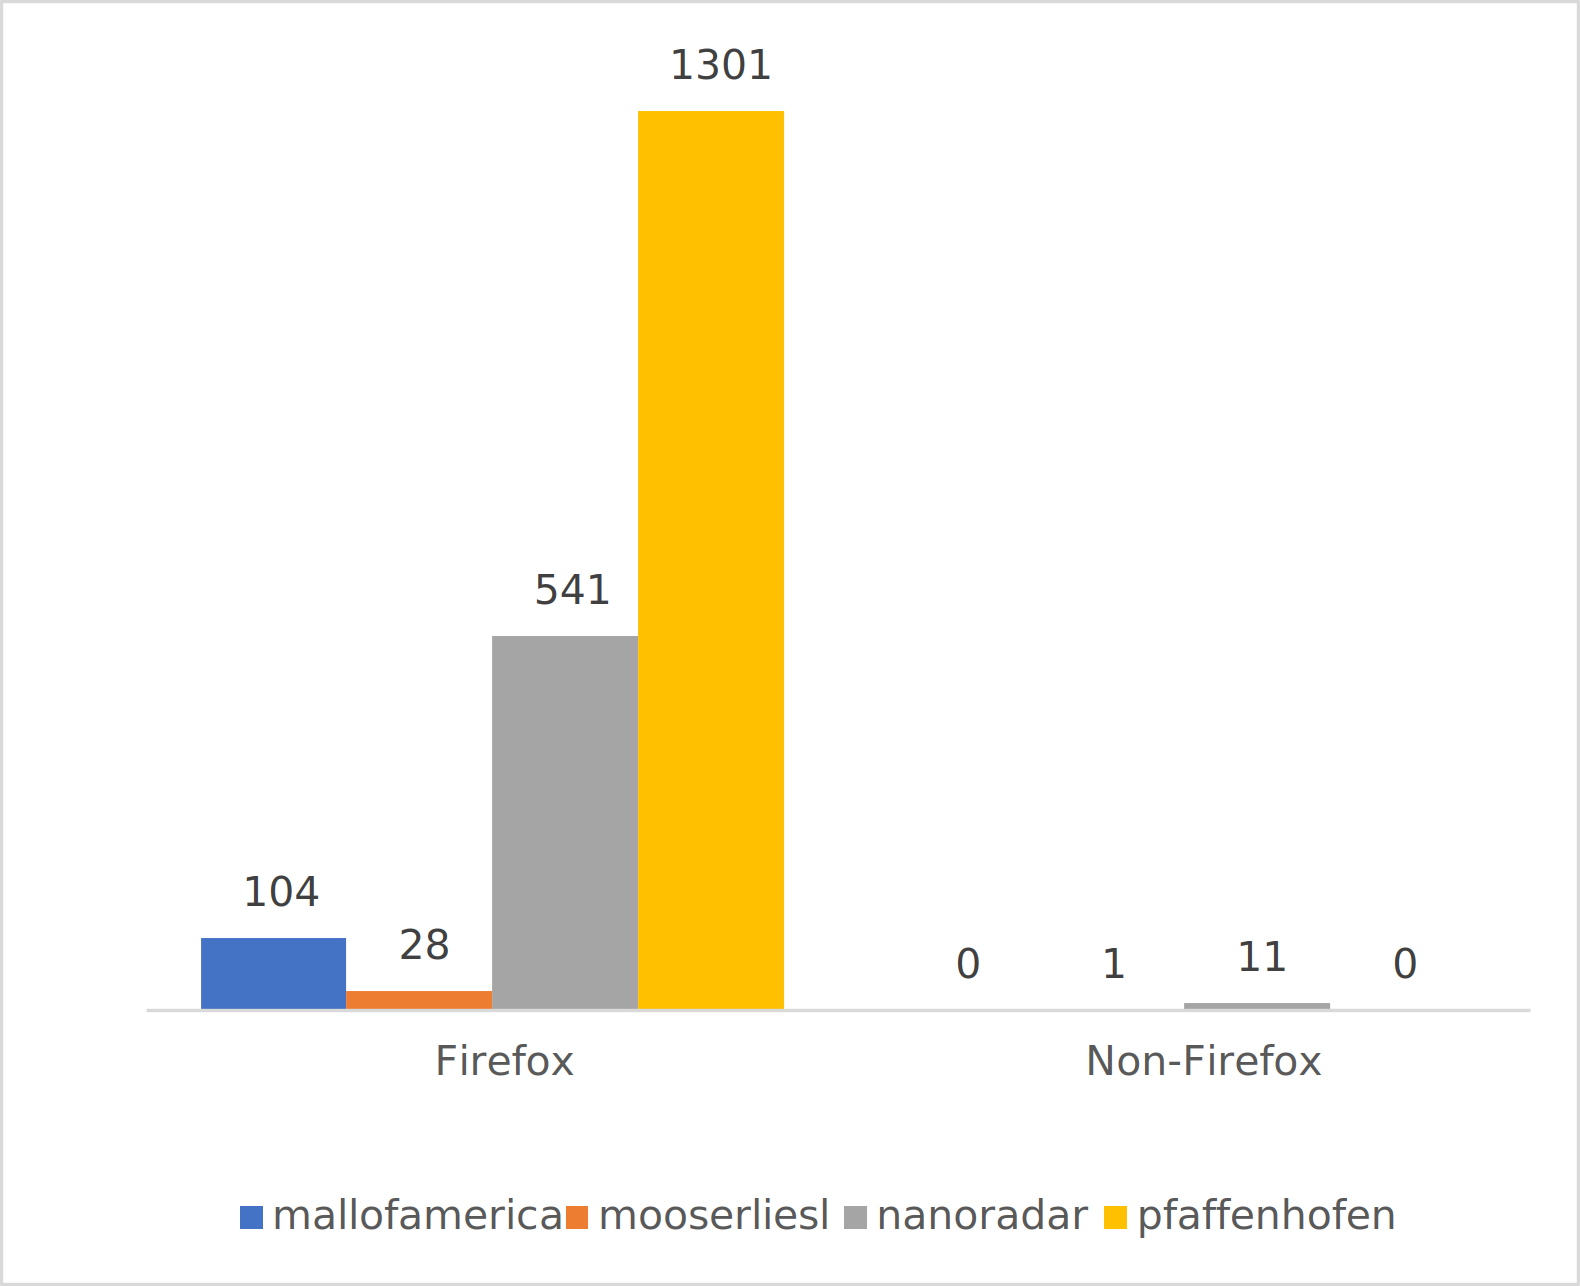
\includegraphics{bilder/bar-chart-test-1.png}}
		}
		\hspace*{\fill}
		\subfloat[]{           
			\resizebox{!}{5cm}{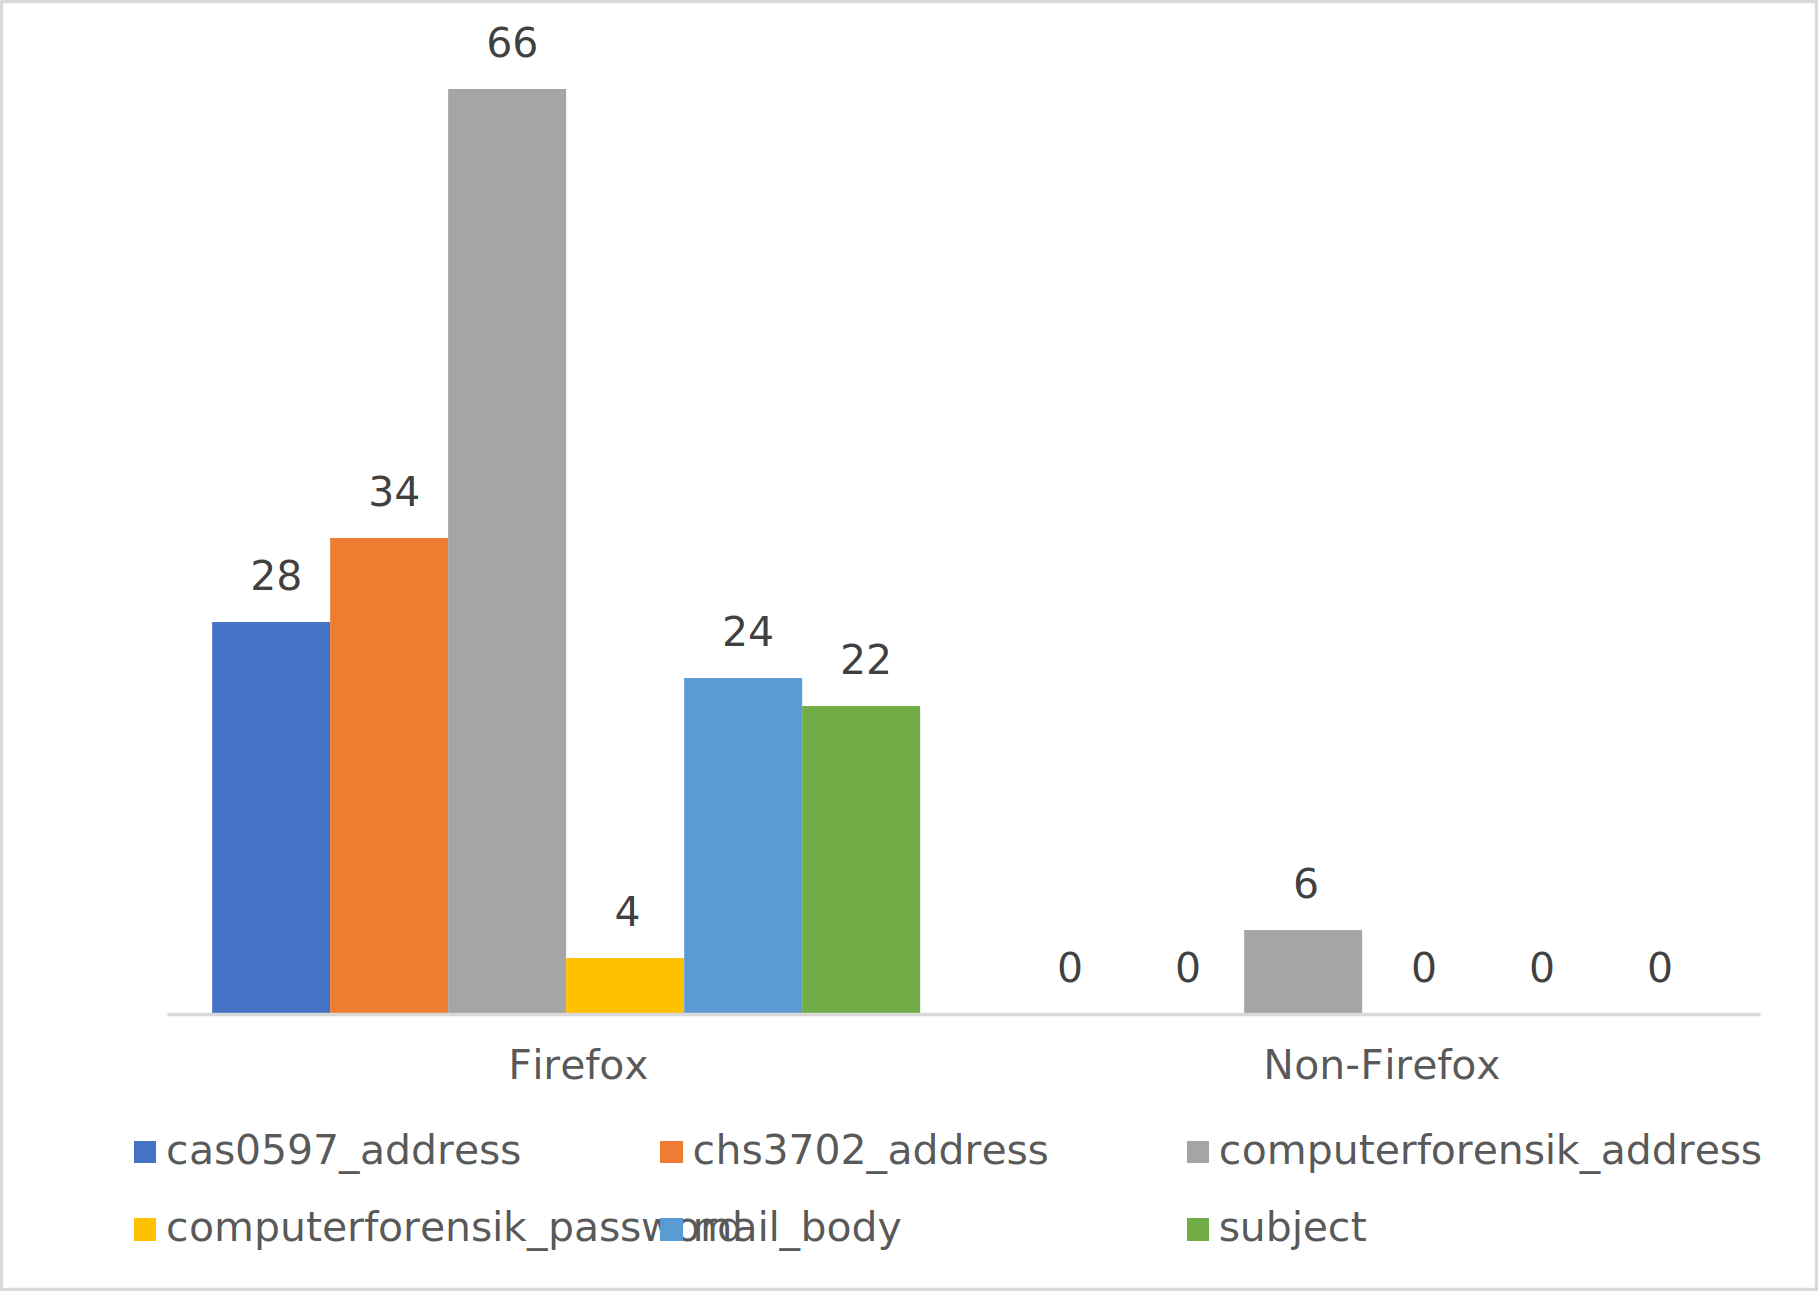
\includegraphics{bilder/bar-chart-test-2.png}}
		}
		\hspace*{\fill}
		\subfloat[]{           
			\resizebox{!}{5cm}{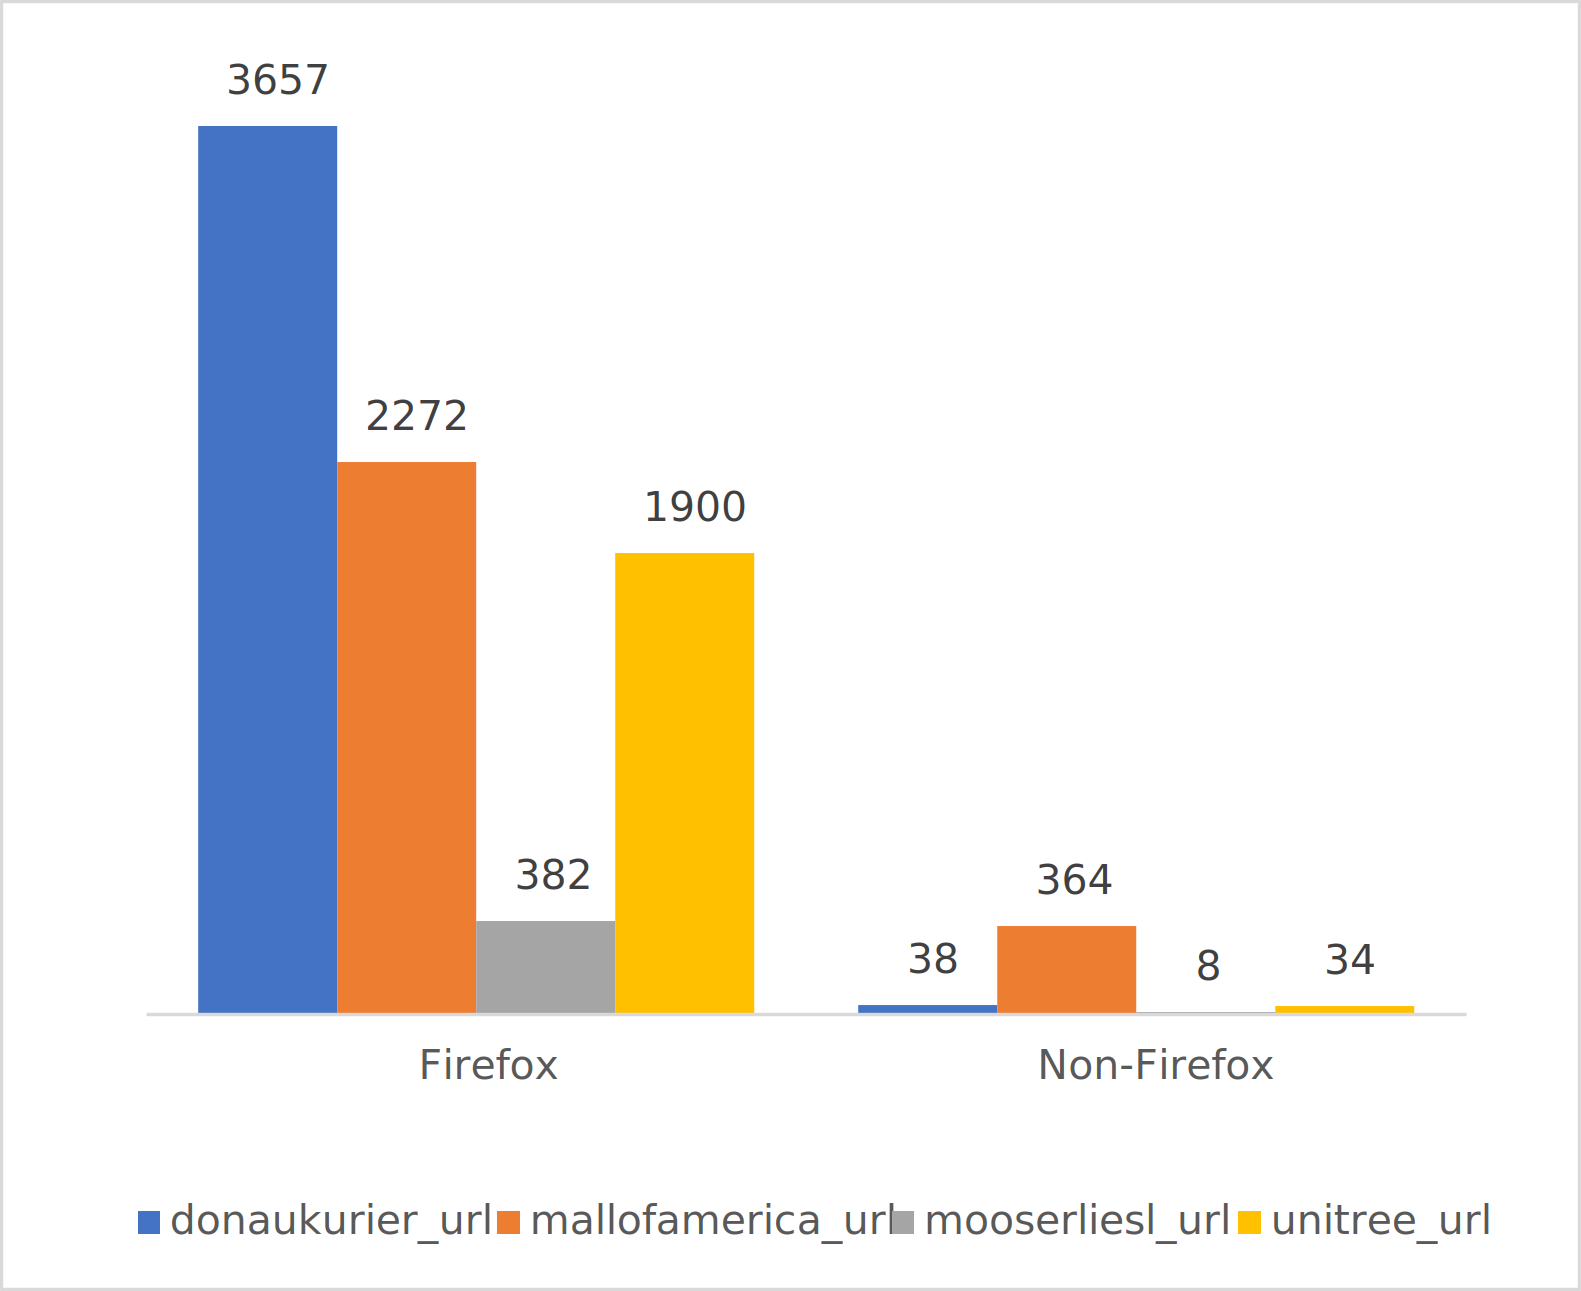
\includegraphics{bilder/bar-chart-test-3.png}}
		}
		\label{chart:final-criteria}  
		\caption{PB Artifacts found in RAM Dump 1}
	\end{figure}

	\captionsetup[subfigure]{labelformat=empty}
	\begin{figure}[h!]
		\small
		\centering	
		\subfloat[]{
			\resizebox{!}{5cm}{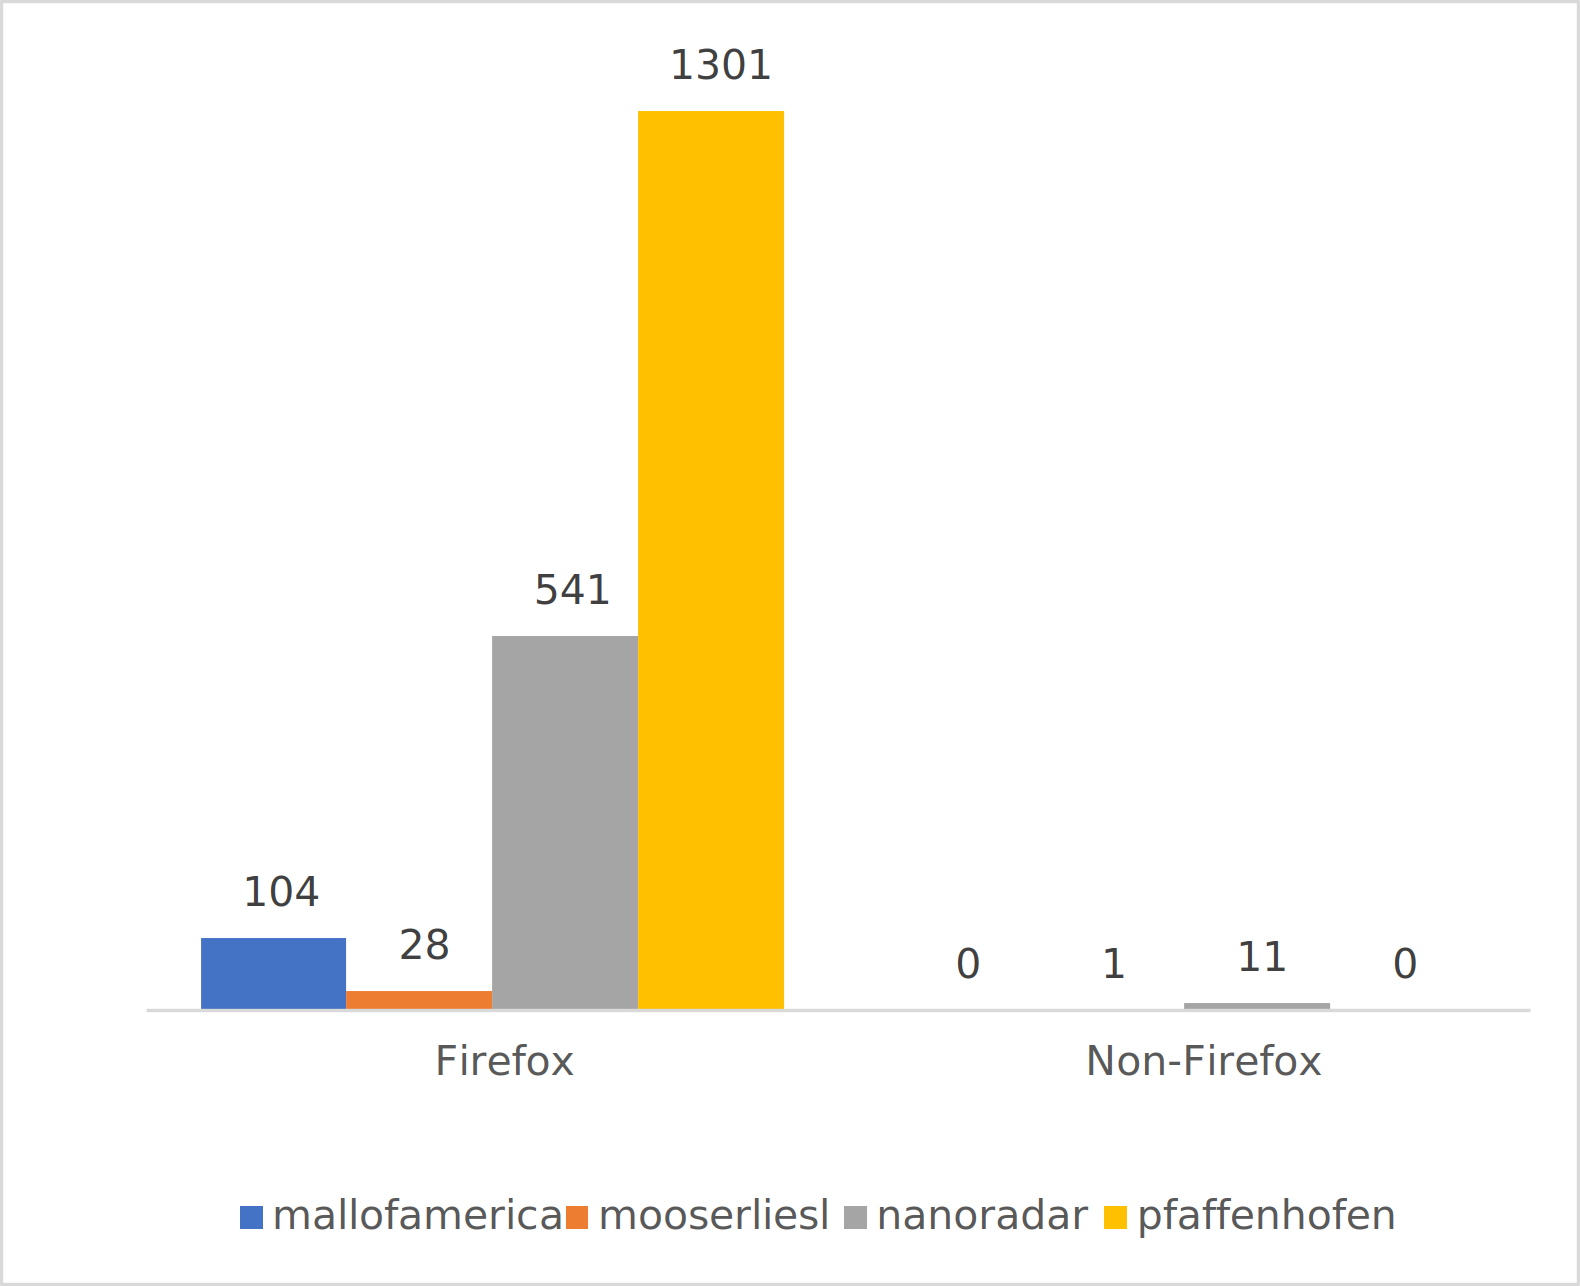
\includegraphics{bilder/bar-chart-test-1.png}}
		}
		\hspace*{\fill}
		\subfloat[]{           
			\resizebox{!}{5cm}{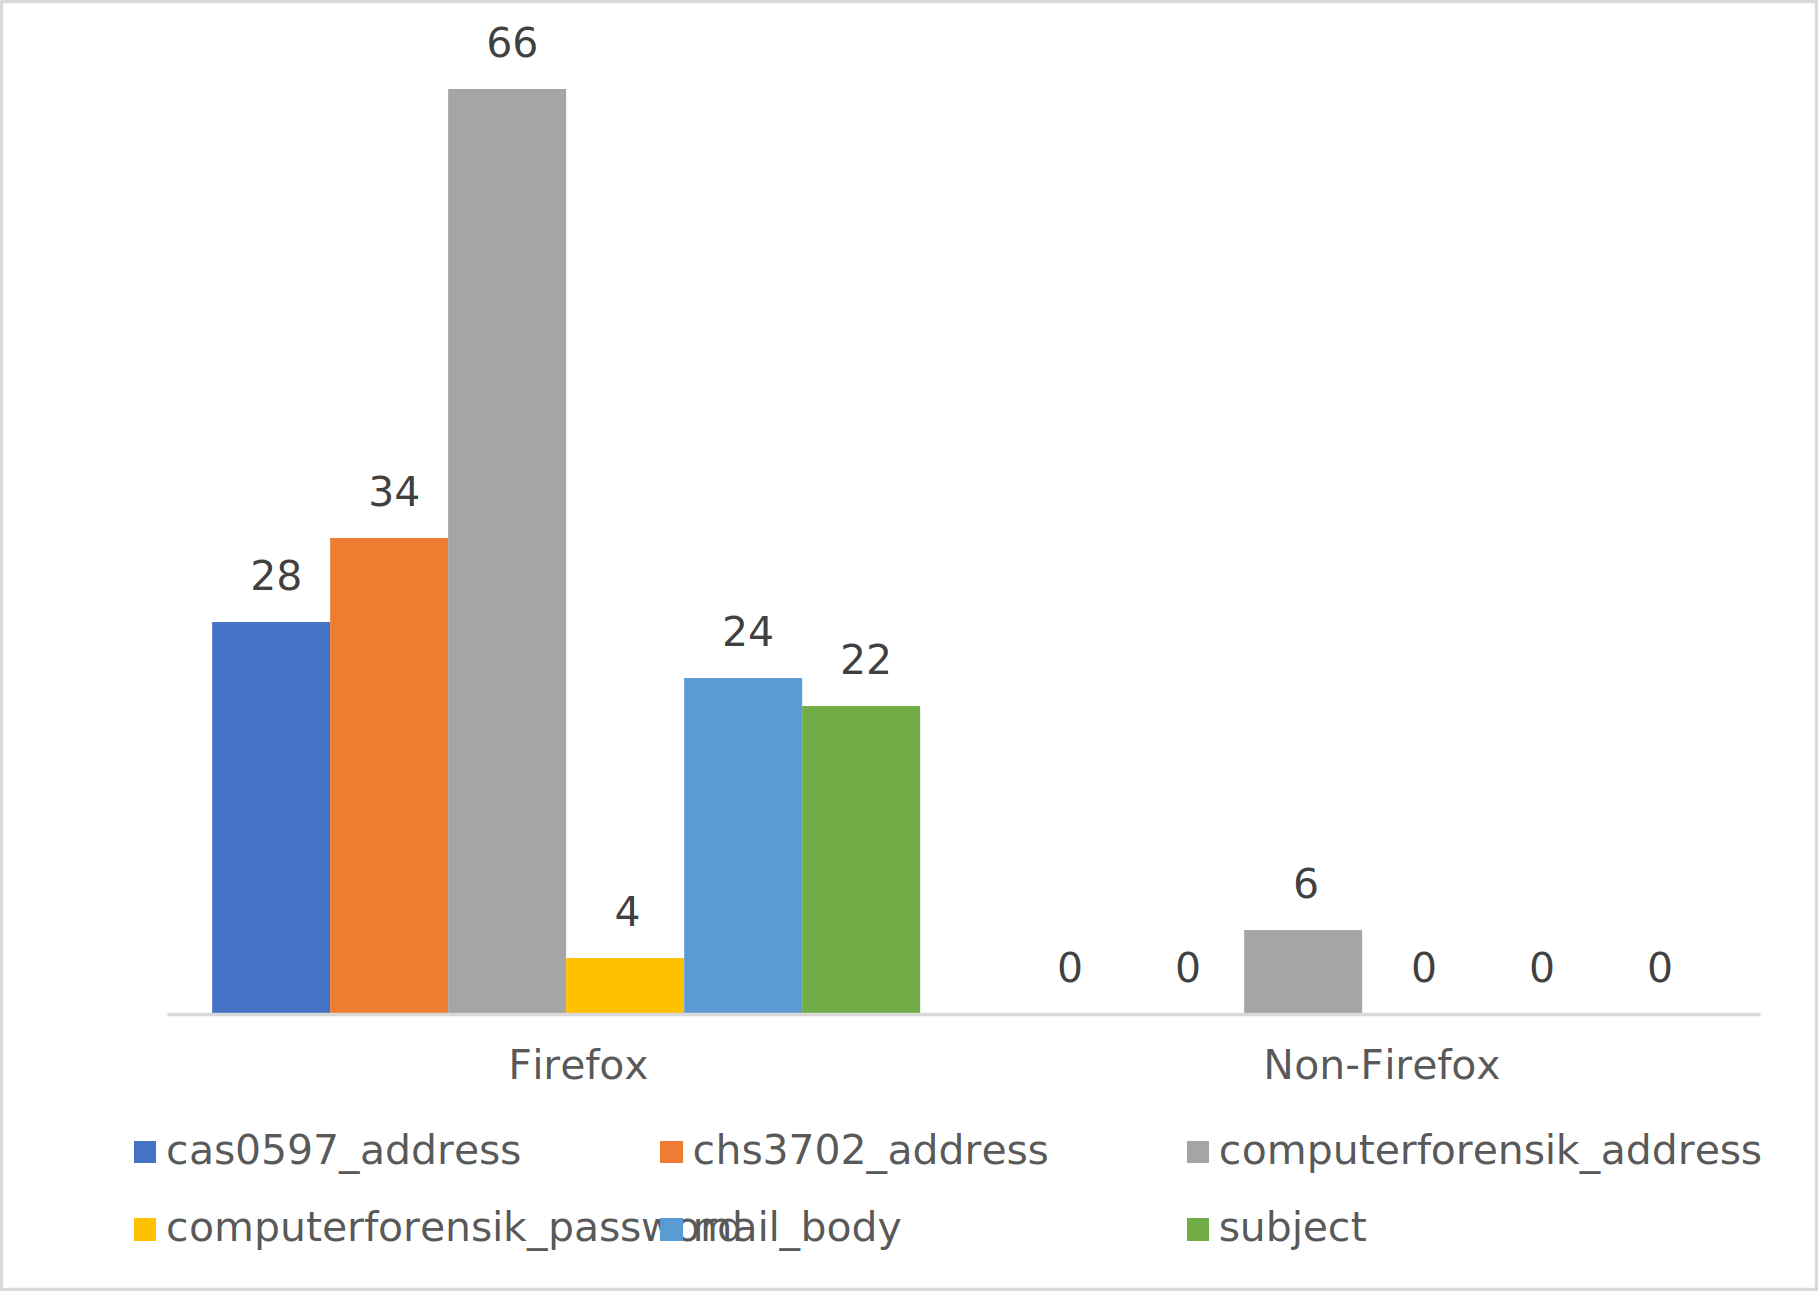
\includegraphics{bilder/bar-chart-test-2.png}}
		}
		\hspace*{\fill}
		\subfloat[]{           
			\resizebox{!}{5cm}{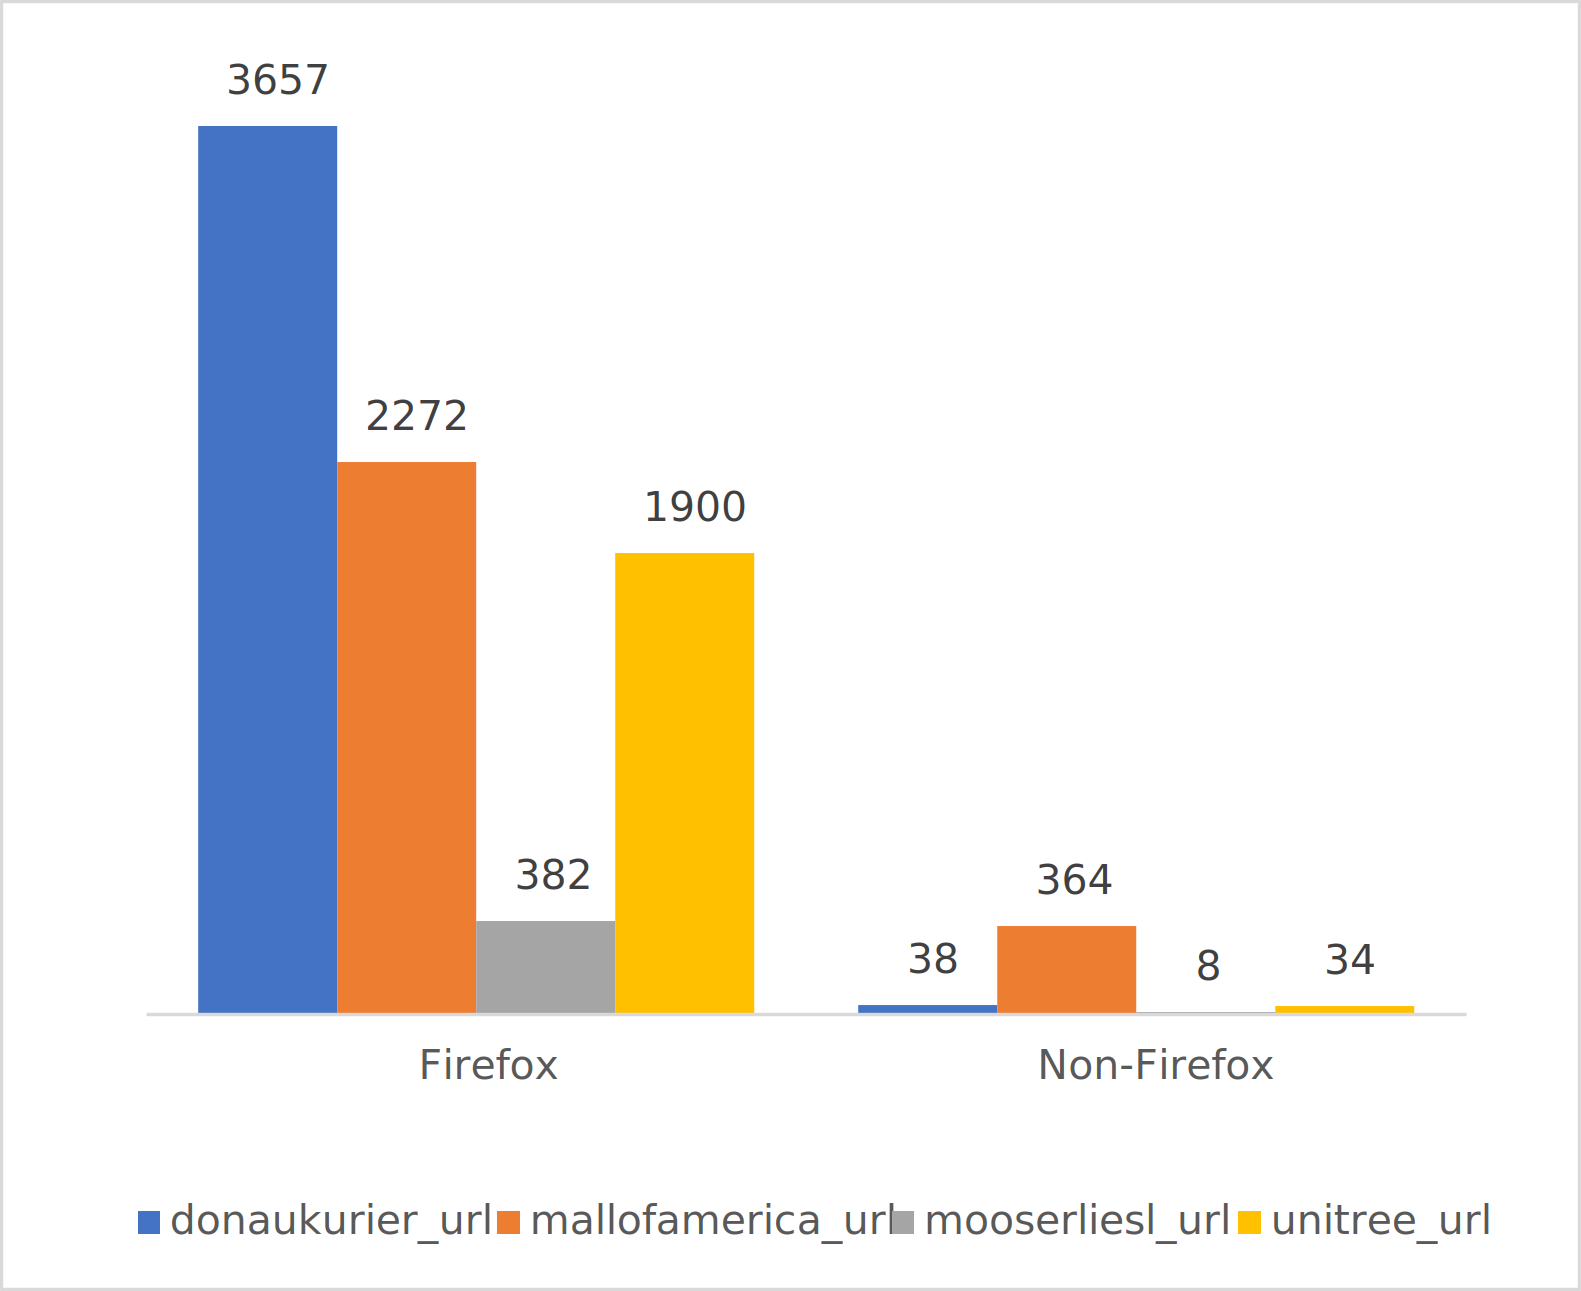
\includegraphics{bilder/bar-chart-test-3.png}}
		}
		\label{chart:final-criteria}  
		\caption{PB Artifacts found in RAM Dump 2}
	\end{figure}
	
	\captionsetup[subfigure]{labelformat=empty}
	\begin{figure}[h!]
		\small
		\centering	
		\subfloat[]{
			\resizebox{!}{5cm}{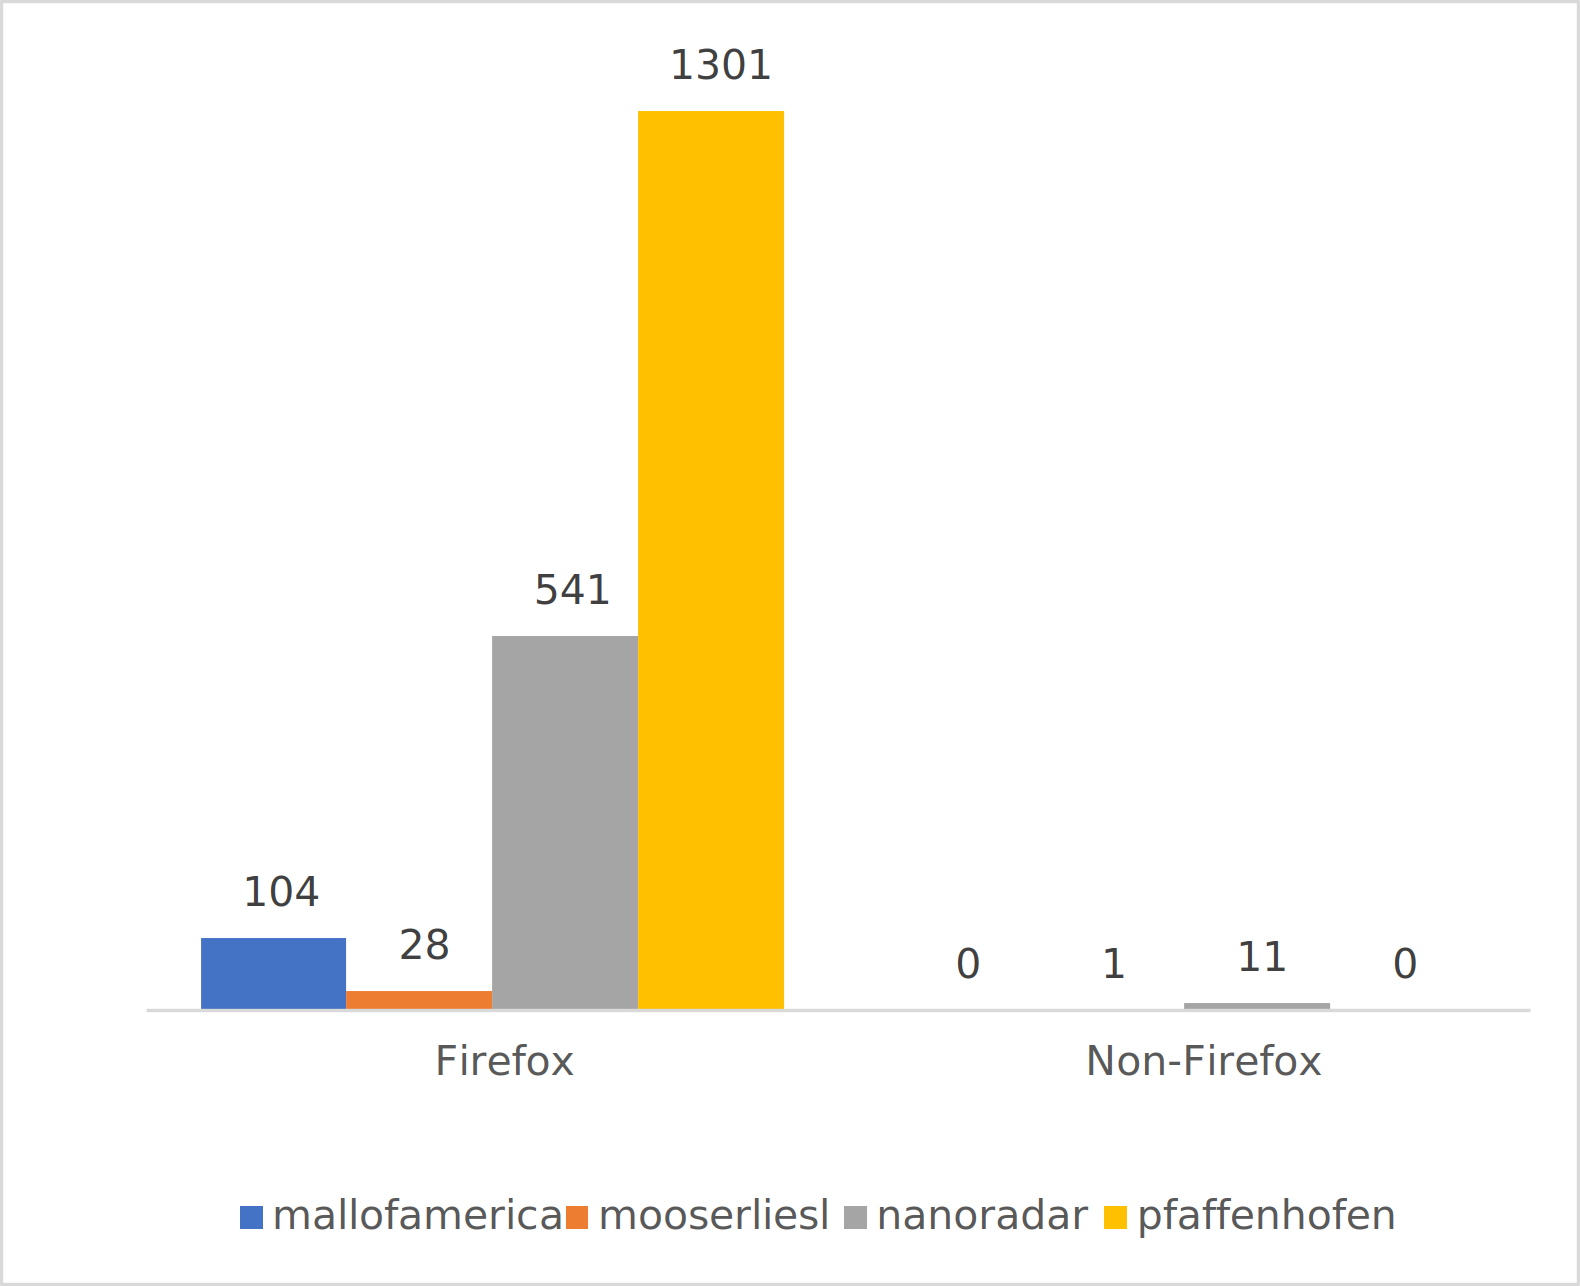
\includegraphics{bilder/bar-chart-test-1.png}}
		}
		\hspace*{\fill}
		\subfloat[]{           
			\resizebox{!}{5cm}{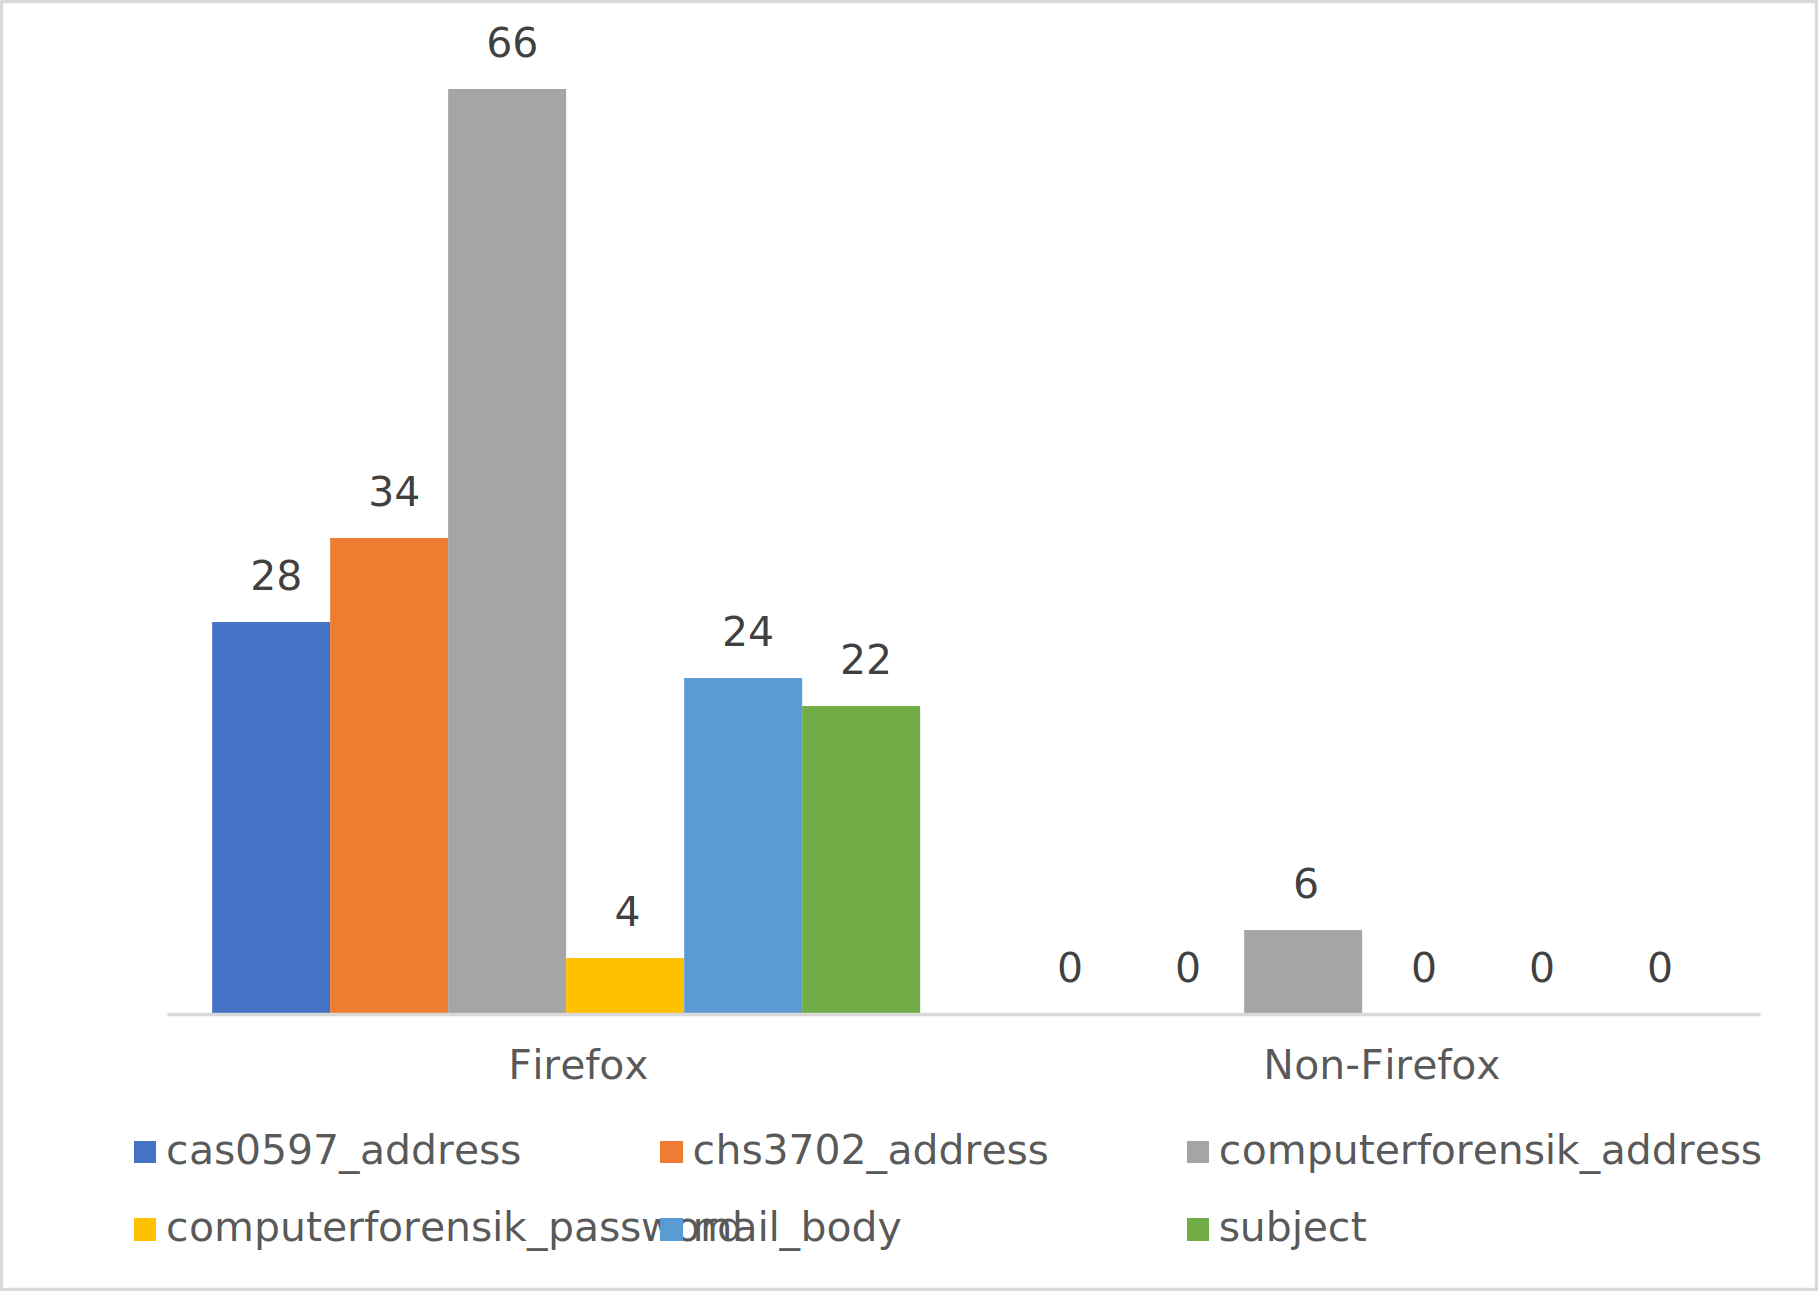
\includegraphics{bilder/bar-chart-test-2.png}}
		}
		\hspace*{\fill}
		\subfloat[]{           
			\resizebox{!}{5cm}{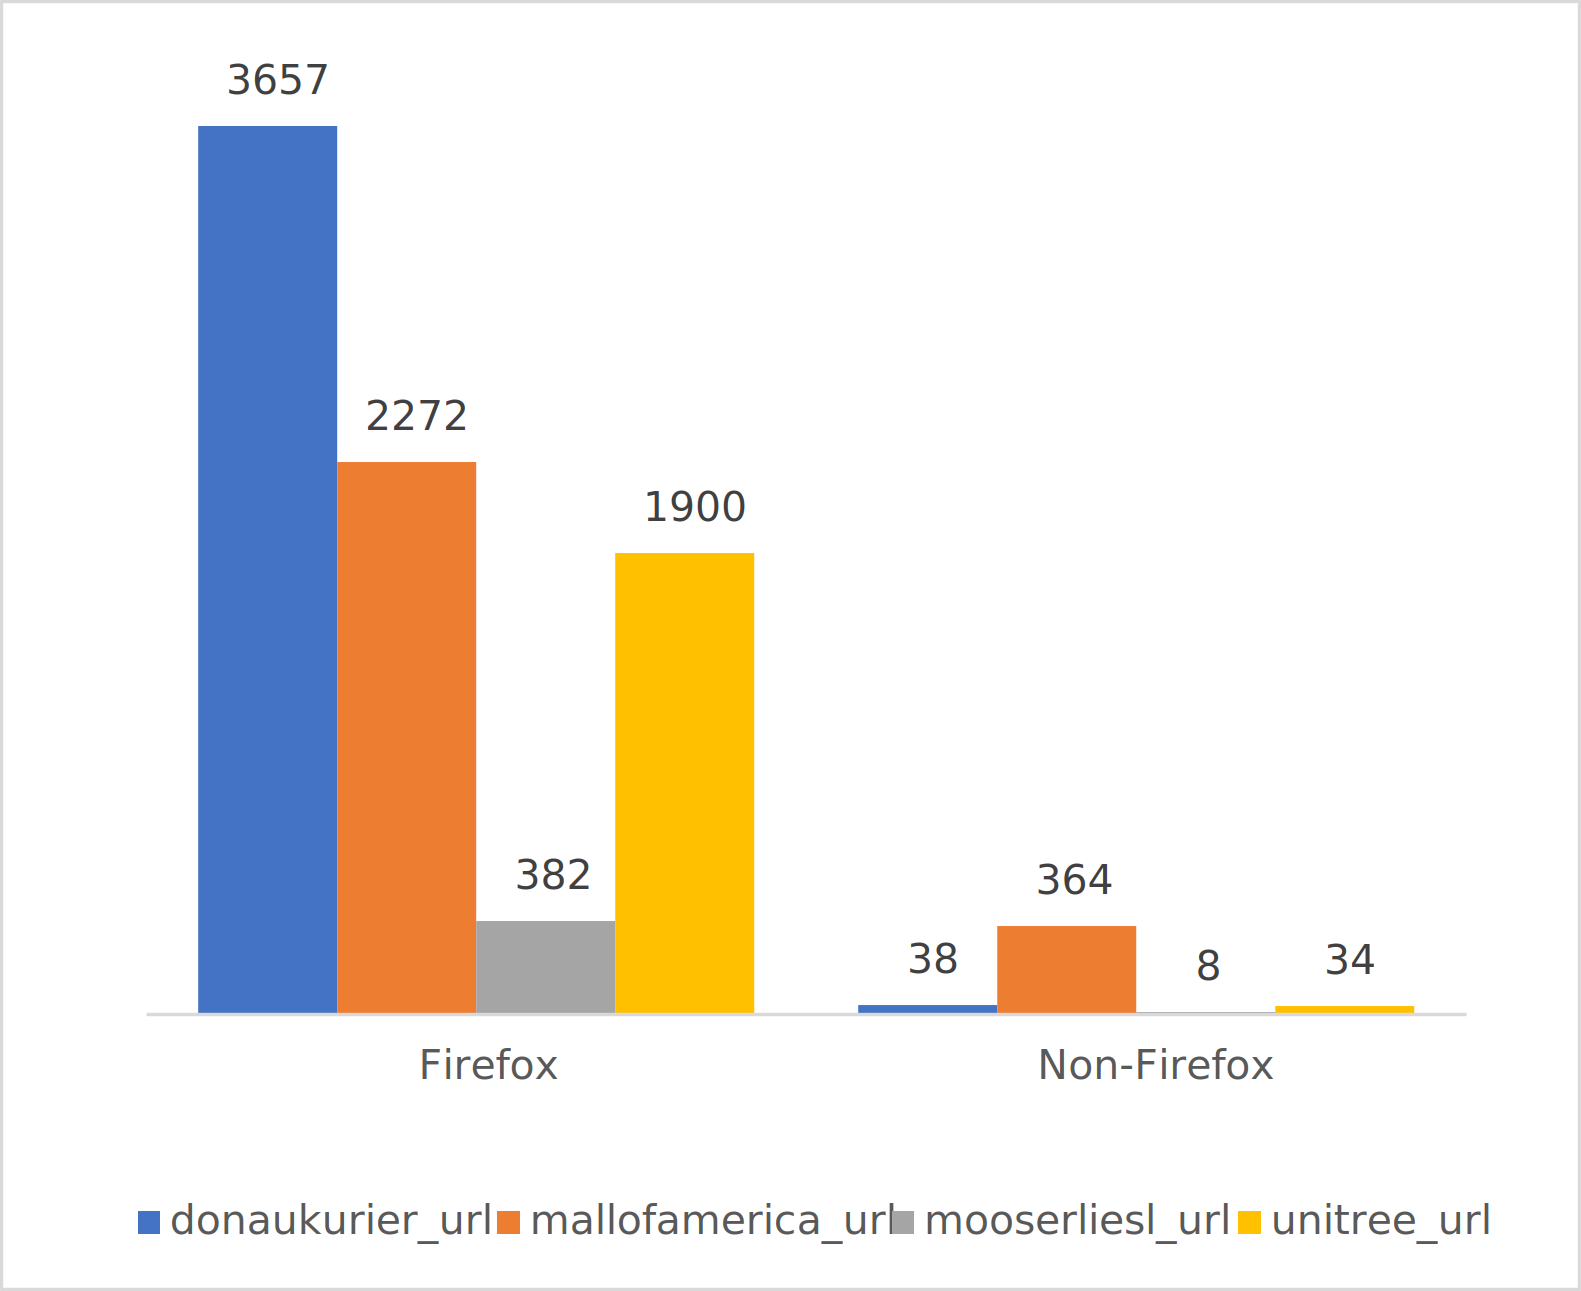
\includegraphics{bilder/bar-chart-test-3.png}}
		}
		\label{chart:final-criteria}  
		\caption{PB Artifacts found in RAM Dump 3}
	\end{figure}
		
	\begin{figure}[h!]
		\resizebox{\linewidth}{!}{\includegraphics{bilder/stacked-bar-chart-test.png}}
		\label{chart:final-criteria}  
		\caption{Comparison of found PB artifacts between RAM Dumps}
	\end{figure}


\section{Tor}

\subsection*{Uncommon Locations}

\subsubsection*{Qualitative Analyse}

o Autopsy: \cite{Muir.2019}
	•	Configuration files, downloaded files, and browserrelated data are recoverable from the file system.
	•	Significant data-leakage from the browsing session occurred: HTTP header information, titles of web pages and an instance of a URL were found in registry files, system files, and unallocated space.



o RAM-Analyse nach \cite{Muir.2019}:
	•	Live-Analyse identifiziert auch nach dem Schließen und Deinstallieren des Browsers und Abmelden des Benutzers Spuren von Tor-Prozessen, einschließlich des absoluten Pfads zur Browser-Executable, des Benutzernamens und des Geräts, von dem es ausgeführt wurde.
	•	The data-leakage contained the German word for ’search’ in reference to a Google search. This hints at the locale of the Tor server used to exit the network (exit relay).

o RAM-Analyse nach \cite{Hariharan.2022}:
	o	process was found to be firefox.exe
	o	pslist and pstree: parent process was shown 
	o	Belkasoft Ram Capturer: retrieve information about facebook
	o	Cmdline: file path of the browser “E:/TorBrowser/Browser/firefox.exe” + name of process tor.exe and firefox.exe
	o	Dlllist: DLL files of the executable files were not captured
	o	Netscan: tor.exe + obfs4proxy.exe -> showed “LISTENING” connections to nonstandardized ports as output.
	Yarascan: was able to retrieve all the browsing sessions
o RAM-Analyse nach \cite{Sajan.2021} mit Volatility
	•	process list extracted from the memory
	•	registry hives been extracted from the memory dump
	•	threads were extracted: “D:/VolatilityWorkbench/volatility.exe”–plugins=”D:/VolatilityWorkbench/profiles” pslistfilename =”C:/Users/username/Desktop/tor.raw” –profile=Win10x64 17763 –kdbg=0xf807606ac5e0
	•	Handles: resources used by the process 5672
	•	Dlls: These dlls can be found from prefetch file --> Can be found in “prefetch” file -> Analyzed with “winprefetchview”
	•	Places.sqlite: SQLite viewer has been used to recover bookmarks and frequently visited sites even after uninstalling the application
	•	Visited Websites: Using keyword search in Dump’s Hex

o Registry:
	> Shellactivites (siehe Firefox) \cite{Muir.2019}: instance of a URL were found in registry file
	> \cite{Nelson.2020} The userassist key is located in the NTUSER.dat hive of the
		 -> Registry and indicates the execution path of the program, as well as the number of times the program was executed 

\subsubsection*{Quantitative Zusammenfassung}



\section{Chrome}

\subsection*{Uncommon Locations}

o Autopsy Keyword-Suche: 
	> Chrome and Edge produced five artefacts as reported by both tools. (FTK, Autopsy) \cite{Gabet.2018}
		--> Artefakte werden nicht genannt!
	> only two temporary files (Figure 7) were recovered with Minitool Power Data Recovery but it was a dead end; Location: appdata/…/Chrome/…/ Preferences/RF1533fa.TMP \cite{Fayyad.2021}
	> pagefile.sys file showed no traces at all \cite{Said.2011}
	

\section{Brave}